El problema de tres cuerpos interactuando en campos gravitacionales ha sido uno de gran análisis desde hace más de 300 años ya que la dinámica de éste tiene comportamientos que distan de ser obvios. Aún en el caso más simplificado, o sea, el problema circular de tres cuerpos (PC3C), presenta alta sensibilidad a las condiciones iniciales, varios puntos de equilibrio, órbitas periódicas y semiperiódicas y, en general, una rica dinámica. Además, el PC3C tiene únicamente dos grados de libertad, lo cuál permite un estudio y una representación gráfica mucho más clara respecto al caso general. Ésto motiva el uso de las herramientas desarrolladas en el capítulo \ref{chap:jt_indicators}. Para ésto es necesario explorar un poco la estructura del problema; encontrar sus puntos de equilibrio, sus singularidades y las ``zonas interesantes'' del espacio fase.

El caso general se plantea de manera estándar bajo el potencial gravitacional de Newton entre pares de cuerpos 
\begin{align}
 U_{M_1}(\mathbf{r}_1,\mathbf{r}_2,\mathbf{r}_3) &= -G \frac{M_1 M_2}{r_{1,2}} - G \frac{M_1 m_3}{r_{1,3}}, \\
 U_{M_2}(\mathbf{r}_1,\mathbf{r}_2,\mathbf{r}_3) &= -G \frac{M_2 M_1}{r_{2,1}} - G \frac{M_2 m_3}{r_{2,3}}, \\
 U_{M_3}(\mathbf{r}_1,\mathbf{r}_2,\mathbf{r}_3) &= -G \frac{m_3 M_1}{r_{3,1}} - G \frac{m_3 M_2}{r_{3,2}},
 \label{eq:3body_potential}
\end{align}

con $G$ la constante de gravitación universal, $\mathbf{r}_i = x_i \hat{\imath} + y_i \hat{\jmath} + z_i \hat{k}$ la posición de la i-ésima partícula, $M_i$ su masa y $r_{i,j} = \norm{ \mathbf{r}_i - \mathbf{r}_j}$ la distancia entre las partículas $M_i$ y $M_j$\footnote{Notemos la simetría $r_{i,j} = r_{j,i}$, aunque $\mathbf{r}_{i,j} = \mathbf{r}_i - \mathbf{r}_j = \mathbf{r}_j - \mathbf{r}_i  = - \mathbf{r}_{j,i}$.}. 

La energía cinética del problema se define de manera usual 
\begin{equation}
 T(\dot{\mathbf{r}}_1,\dot{\mathbf{r}}_2,\dot{\mathbf{r}}_3) = \frac{1}{2} \sum_{i=1}^3 M_i \dot{r}_i^2,
 \label{eq:3body_kinetic}
\end{equation}
y define un sistema de 6 ecuaciones acopladas dadas por la segunda ley de Newton
\begin{equation}
 M_i \ddot{\mathbf{r}_i} = - G M_i \sum_{j\neq i} \frac{M_j}{r_{i,j}^2} \hat{\mathbf{r}}_{i,j},
 \label{eq:3body_eqs_motion}
\end{equation}
con $\hat{\mathbf{r}}_{i,j} = \frac{\mathbf{r}_{i,j}}{r_{i,j}}$ un vector unitario en la dirección de $\mathbf{r}_{i,j}$.

Hasta aquí, ninguna restricción ha sido impuesta, y encontrar simetrías para reducir los grados de libertad no es fácil. Sin embargo, para el problema restringido de tres cuerpos uno supone que una de las partículas es mucho menos masiva que las otras dos y, por tanto, las dos más grandes se mueven como si la tercera no existiera. Vale la pena estudiar primero el caso de dos cuerpos, ver la dinámica entre ellos y luego regresar a la tercer partícula bajo la influencia de estos dos. 

\section{Problema de dos cuerpos}
\label{sec:2body_problem}
Dadas que $M_1$ y $M_2$ son los cuerpos primarios y $m_3$ es despreciable, la dinámica de éstos queda definida por
\begin{equation}
 \mathbf{F}_1(\mathbf{r}_1,\mathbf{r}_2) = M_1 \ddot{\mathbf{r}}_1 = -G \frac{M_1 M_2}{r_{1,2}^2} \hat{\mathbf{r}}_{1,2}.
 \label{eq:2body_eqs_motion}
\end{equation}
Como $\hat{\mathbf{r}}_{1,2} = - \hat{\mathbf{r}}_{2,1}$ entonces $\mathbf{F}_2 = -\mathbf{F}_1$, lo cual es equivalente a la tercera ley de Newton. Se tomará como referencia el capítulo 3 del libro de mecánica analítica de Goldstein \cite{Goldstein2007} para obtener las soluciones de este problema. Por comodidad llamaremos a $\mathbf{r}_{1,2}$ simplemente $\mathbf{R}$ y, en términos de ésta, se puede plantear el problema de Kepler, que describe la aceleración relativa
\begin{equation}
 \ddot{\mathbf{R}} = \ddot{\mathbf{r}}_1 - \ddot{\mathbf{r}}_2 = -G \frac{M_1 + M_2}{R^2} \hat{\mathbf{R}} = - \frac{\beta}{R^2}\hat{\mathbf{R}},
 \label{eq:kepler_problem}
\end{equation}
con $\beta = G \left(M_1 + M_2 \right)$. Multiplicando (\ref{eq:kepler_problem}) por la masa reducida $\gamma := \frac{M_1 M_2}{M_1+M_2}$ obtenemos las ecuaciones de movimiento de la fuerza relativa de $M_1$ respecto a $M_2$.

El problema de Kepler conserva el momento angular $\mathbf{L} := \mathbf{R} \times \mathbf{p}$, ya que
\begin{equation}
 \frac{d\mathbf{L}}{dt} = \frac{d}{dt}\left(\mathbf{R} \times \gamma\dot{\mathbf{R}} \right) = \gamma\dot{\mathbf{R}} \cancelto{0}{\times}\dot{\mathbf{R}} + \mathbf{R} \times \gamma \ddot{\mathbf{R}} = - \mathbf{R} \cancelto{0}{\times} G\frac{\gamma \beta}{r^2}\hat{\mathbf{R}} = 0
\end{equation}
y, por tanto, $\mathbf{L} = \text{constante}$. Así, $\mathbf{R}$ y $\dot{\mathbf{R}}$ son perpendiculares a $\mathbf{L}$ y por tanto, viven en un plano que por comodidad se escoge en $xy$. 

Una mejor descripción del movimiento se puede obtener en coordenadas polares, donde
\begin{align}
 \hat{R} &= \cos \theta \hat{\imath} + \sin \theta \hat{\jmath} \nonumber, \\
 \hat{\theta} &= -\sin \theta \hat{\imath} + \cos \theta \hat{\jmath},
 \label{eq:polar_transformation}
\end{align}
con $z=0$ en el plano de movimiento. 

Haciendo la regla de la cadena obtenemos las expresiones para  $\mathbf{R}$,$\dot{\mathbf{R}}$ y $\ddot{\mathbf{R}}$
\begin{align}
 \mathbf{R} &= R \cos \theta \hat{\imath} + R \sin \theta \hat{\jmath} = R \hat{R}, \\
 \dot{\mathbf{R}} &= \left( \dot{R} \cos \theta - R \sin \theta \dot{\theta} \right) \hat{\imath} + \left( \dot{R} \sin \theta + R \cos \theta \dot{\theta} \right) \hat{\jmath} = \dot{R}\hat{R} + R \dot{\theta} \hat{\theta}, \\
 \ddot{\mathbf{R}} &= \left(\ddot{R} - R \dot{\theta}^2 \right) \hat{R} + \left( R \ddot{\theta} + 2 \dot{R}\dot{\theta} \right) \hat{\theta}.
 \label{eq:motion_polar_variables}
\end{align}

En este sistema de coordenadas es fácil ver que
\begin{equation}
 L = \norm{ \mathbf{L} } = \norm{ \mathbf{R} \times \gamma \dot{\mathbf{R}} } = \norm{ \left( R \hat{R} + 0 \hat{\theta} + 0 \hat{k} \right) \times \left( \dot{R} \hat{R} + R \dot{\theta} \hat{\theta} + 0\hat{k} \right) } = \gamma R^2 \dot{\theta},
\end{equation}
obteniendo así
\begin{equation}
\dot{\theta}(R) = \frac{L}{\gamma R^2}.
\label{eq:2body_ang_vel}
\end{equation}

Con (\ref{eq:motion_polar_variables}) podemos replantear (\ref{eq:kepler_problem}) y obtener las ecuaciones de movimiento en las nuevas coordenadas
\begin{align}
 R \ddot{\theta} + 2 \dot{R} \dot{\theta} &= 0, \\
 \ddot{R} - R \dot{\theta}^2 &= -\frac{\beta}{R^2}.
 \label{eq:2body_eqs_motion_polar}
\end{align}
Notemos que la primera queda resuelta por (\ref{eq:2body_ang_vel}) mientras que la segunda, usando que $\dot{R} = \frac{d R}{d\theta} \dot{\theta}$, se convierte en
\begin{align*}
 \frac{d^2 R}{d \theta^2} \dot{\theta}^2 + \frac{dR}{d\theta} \ddot{\theta} - R \dot{\theta}^2 = - \frac{\beta}{R^2},
\end{align*}
donde 
\begin{equation*}
 \ddot{\theta} = -\frac{2L}{\gamma R^3}\dot{R} = -\frac{2L}{\gamma R^3} \frac{dR}{d\theta}\dot{\theta} = - \frac{2L^2}{\gamma^2 R^5} \frac{dR}{d\theta}.
\end{equation*}
Ésto y (\ref{eq:2body_ang_vel}) se sustituyen en  (\ref{eq:2body_eqs_motion_polar}) para obtener
\begin{equation*}
 \frac{L^2}{\gamma^2 R^4}\left( \frac{d^2R}{d\theta^2} - \frac{1}{R} \left(\frac{dR}{d\theta} \right)^2 -R \right) = - \frac{\beta}{R^2}.
\end{equation*}

Finalmente, si hacemos $u(R) := \frac{1}{R}$, se simplifica la ecuación diferencial a
\begin{equation}
 \frac{d^2u}{d\theta^2} + u = \frac{\beta \gamma^2}{L^2},
\end{equation}

que no es más que un oscilador armónico con forzamiento constante $\frac{\beta \gamma^2}{L^2}$. Obtenemos explícitamente la solución para $u$:

\begin{equation*}
 u(\theta) = \frac{\beta \gamma^2}{L^2} \left( 1 + e \cos (\theta - \theta_0 ) \right) ,
\end{equation*}
\begin{equation}
 \therefore R(\theta) = \frac{L^2}{\beta \gamma^2 \left(1 + e \cos (\theta - \theta_0) \right)}.
 \label{eq:2body_solution}
\end{equation}

%Cómo obtenemos explícitamente la forma de $e$ y de $\theta_0$? 
%Por qué esta ecuación representa una sección cónica en polares? Debería simplemente decirlo y citar algún texto? Chance sí...  

Ésta es la distancia relativa que tienen $M_1$ y $M_2$ en función del ángulo $\theta$. Notemos que (\ref{eq:2body_solution}) representa diferentes secciones cónicas en coordenadas polares y depende de la eccentricidad $e$ únicamente.

\section{Problema circular de tres cuerpos}
\label{sec:R3BP}

Ahora se tomará a la tercer partícula considerando que sea mucho más pequeña que las otras dos, i.e., $m_3 \ll M_2 \leq M_1$. Así, $m_3$ es ignorada en la dinámica de $M_2$ y $M_1$ y, por tanto, la solución para los cuerpos primarios es la desarrollada en la sección anterior. Sólo queda estudiar la dinámica de $m_3$ en relación a $M_1$ y $M_2$ para describir completamente al problema.

Para el caso circular, se toma $e = 0$ y, así, la distancia entre las masas primarias
\begin{equation}
 R = \frac{L^2}{\gamma^2 \beta}
 \label{eq:3body_restricted_solution}
\end{equation} 
es constante.

Con ésto, la velocidad angular también es constante y, con (\ref{eq:3body_restricted_solution}) en (\ref{eq:2body_ang_vel}), se plantea
\begin{equation}
 \Omega := \dot{\theta} = \sqrt{ \frac{\beta R}{R^4} } = \sqrt{\frac{G \left(M_1 + M_2 \right)}{R^3}}.
 \label{eq:3body_ang_velocity}
\end{equation}

Para la dinámica de $m_3$ conviene establecer un marco de referencia en rotación donde $M_1$ y $M_2$ estén en reposo. Dicha rotación tendrá velocidad angular $\Omega$ y estará basada en el centro de gravedad entre las dos. En el apéndice \ref{chap:rotating_frames} se muestra la transformación para dicho sistema. Específicamente aparecen la aceleración de Coriolis, la aceleración centrífuga, y la aceleración inercial que es cero en este caso, dado que el origen es el centro de gravedad entre $M_1$ y $M_2$. Dichas fuerzas, aunque se llamen ficticias, no aparecen de la nada. Éstas son el resultado de la rotación de las masas primarias alrededor del centro de masa y, por tanto, deberán hacer que el sistema siga siendo conservativo. 

%Recordemos, de la sección  \ref{sec:ficticious_forces}, que un sistema de referencia en rotación traerá algunas fuerzas ficticias descritas por (\ref{eq:rotating_constant_acceleration}), más específicamente la aceleración de Coriolis y la aceleración centrípeta. Como en este caso el sistema está centrado en el centro de gravedad de $M_1$ y $M_2$, la aceleración inercial del sistema será nula en todo momento.

Las ecuaciones de movimiento para $m_3$ en el sistema en rotación son
\begin{equation}
 \ddot{\mathbf{r}} + 2\mathbf{\Omega} \times \dot{\mathbf{r}} = - \nabla V(\mathbf{r}),
 \label{eq:3body_restricted_acceleration}
\end{equation}
con $\mathbf{r} = (x,y,z)$ la distancia de $m_3$ al centro de gravedad, $\mathbf{R} = \mathbf{r}_1 - \mathbf{r}_2 = (r_1 + r_2,0,0)$ la distancia entre $M_1$ y $M_2$ y
\begin{equation}
 V(r) = \left( -G \frac{M_1}{\norm{\mathbf{r}-\mathbf{r_1}}} - G \frac{M_2}{\norm{\mathbf{r}-\mathbf{r_2}}} - \frac{1}{2} \Omega^2 r^2 \right),
 \label{eq:3body_restricted_potential}
\end{equation} 
que se conoce como \textbf{pseudo-potencial}, ya que si la velocidad es distinta de cero, la fuerza de Coriolis debe ser considerada para la dinámica de la partícula.

Con el afán de reducir el número de parámetros que definen al problema, trabajaremos en unidades especiales tales que 
\begin{align}
 M_1 + M_2 &= 1 \ um, \nonumber \\
 R = r_2 - (-r_1) &= 1 \ ud, \nonumber \\
 \Omega &= 1 \frac{rad}{ut}, \nonumber \\
 \implies G &= 1 \frac{ud^3}{ut^2 \cdot um}. 
 \label{eq:3body_new_units}
\end{align}
Éstas nos permiten además adimensionalizar las ecuaciones de movimiento. Para ésto, es cómodo poner el origen en el centro de masa entre $M_1$ y $M_2$, y a éstas alineadas sobre el eje $x$, así $CM = (0,0) = (-M_1r_1 + M_2r_2, 0)$ obteniendo $-r_1 = -M_2$ y $r_2 =M_1$, ya dividiendo entre las unidades establecidas en (\ref{eq:3body_new_units}). Definimos el parámetro de masa 
\begin{equation*}
 \mu = \frac{M_2}{M_1 + M_2} 
\end{equation*}
con el que podemos replantear todo en términos adimensionales
\begin{align}
 M_1 &= 1 - \mu, \nonumber \\
 M_2 &= \mu, \nonumber \\
 -r_1 &= -\mu, \nonumber \\
 r_2 &= 1 - \mu, \nonumber \\
 G &= 1 \nonumber, \\
 \Omega &= 1.
 \label{eq:3body_adimensional_units}
\end{align}

Así, (\ref{eq:3body_restricted_potential}) se expresa como
\begin{equation}
 V(r) = V(x,y) = -\frac{1 - \mu}{\sqrt{(x + \mu)^2 + y^2}} -  \frac{\mu}{\sqrt{(x - 1 + \mu)^2 + y^2}} - \frac{1}{2} \left(x^2 + y^2 \right)
\end{equation}
y las ecuaciones de movimiento asociadas a (\ref{eq:3body_restricted_acceleration}) son
\begin{align}
 \dot{x} &= v_x, \\
 \dot{y} &= v_y, \\
 \dot{v}_x - 2v_y &=  x - \frac{(1 - \mu) (x+\mu)}{\sqrt{ (x+\mu)^2 + y^2 }^3} - \frac{\mu (x - 1 + \mu) }{\sqrt{(x - 1 +  \mu)^2 + y^2}^3 }, \\ 
 \dot{v}_y + 2v_x &= y \left( 1 - \frac{ 1 - \mu }{\sqrt{(x+\mu)^2 + y^2}^3} - \frac{\mu}{\sqrt{(x - 1 + \mu)^2 + y^2}^3} \right),
 \label{eq:3body_restricted_ eqs_motion}
\end{align}
donde todo queda en términos del único parámetro $\mu$ y el sistema es únicamente de dos grados de libertad, como se mencionó al principio del capítulo. 

Existe una primera integral del sistema si hacemos el producto interno de (\ref{eq:3body_restricted_acceleration}) por $\dot{\mathbf{r}}$, que resulta en 
\begin{align*}
 \ddot{x} \dot{x} + \ddot{y} \dot{y} &= - \pder{V}{x}\dot{x} - \pder{V}{y} \dot{y} \\
 \implies - \frac{1}{2} \left( \dot{x}^2 + \dot{y}^2 \right) &= \int \frac{d V}{dt} = V - C_J 
\end{align*}
\begin{equation}
 \therefore C_J = V + \frac{1}{2}v^2,
 \label{eq:3body_jacobi_constant}
\end{equation}
con $C_J$ la constante de integración que se conoce como constante de Jacobi o energía de Jacobi el cual será útil para el TJ como parámetro para verificar la precisión en las integraciones.

\subsection{Puntos lagrangianos}
\label{sec:lag_points}

Aún sin que el problema sea conservativo si no tomamos en cuenta las fuerzas de Coriolis ya sin ésta la energía mecánica no es una constante de movimiento, vale la pena estudiar las curvas de nivel del pseudo-potencial, o curvas de velocidad cero, ya que éste nos dará una buena intuición sobre cómo será la trayectoria de nuestra partícula. De hecho, los puntos de equilibrio seguirán siéndolo cuando se tome el sistema completo, ya que en éstos la velocidad es cero\footnote{Estos puntos de equilibrio se vuelven órbitas periódicas de velocidad angular constante en el sistema inercial.}. La Figura \ref{fig:3body_pseudo_potential} presenta dichas curvas de nivel, donde se observan tres puntos singulares en el eje alineados a $M_1$ y $M_2$ que se suelen llamar $L_2$,$L_1$ y $L_3$, respectivamente. Otros dos existen para $y \neq 0$ los cuales se conocen como $L_4$ y $L_5$. Éstos cinco reciben el nombre de puntos lagrangianos en honor a los estudios de Lagrange y Euler sobre el tema \cite{Lagrange1867 , Euler1736}.

%FIGURA! 
\begin{figure}[h!]
 \centering
 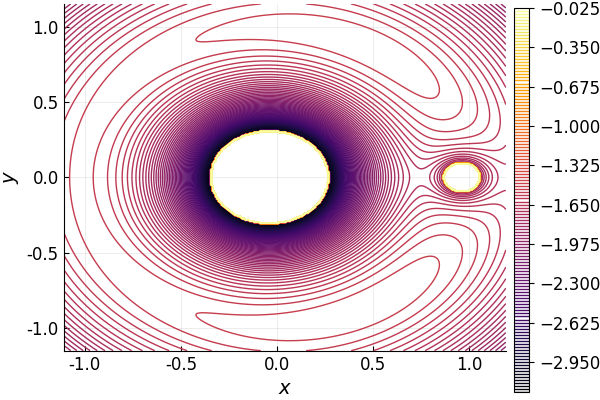
\includegraphics[width=0.8\linewidth]{pseudo_potential}
 \caption{Curvas de nivel para el pseudo-potencial $V(x,y)$ con $\mu = \frac{1}{26}$, $R=1$ y $G=1$ unidades adimensionales.}
 \label{fig:3body_pseudo_potential}
\end{figure}

Siguiendo el desarrollo de \cite{Cornish1998, Widnall2008}, encontraremos dónde están dichos puntos singulares y se hará un análisis de estabilidad de éstos.

Los tres primeros se dan cuando $y=0$, quedando por resolver únicamente cuándo $\dot{v}_x = 0$. Esto plantea una ecuación de quinto grado en $x$ complicada de resolver analíticamente. Sin embargo, cuando $M_1$ es considerablemente más grande que $M_2$, se puede tomar la aproximación a primer orden de $\mu$ y conseguir
\begin{align}
 L_1 &\approx \left( \left[ 1 - \left(\frac{\mu}{3}\right)^{1/3} \right] R , 0 \right) \nonumber, \\ 
 L_2 &\approx \left( \left[ 1 + \left(\frac{\mu}{3}\right)^{1/3} \right] R , 0 \right) \nonumber, \\
 L_3 &\approx \left( -\left[ 1 + \frac{5 \mu}{12} \right] R, 0 \right).
 \label{eq:3body_L123}
\end{align} 

También se pueden obtener estos valores numéricamente para cualquier $\mu$, pero hace un poco más complicado el análisis de estabilidad ya que no se consiguen en función de $\mu$. Sin embargo, como se observa en la Figura \ref{fig:3body_pseudo_xaxis}, para $\mu = \frac{1}{26}$ sí se llega a notar la diferencia.

%FIGURA!
\begin{figure}[h!]
 \centering
 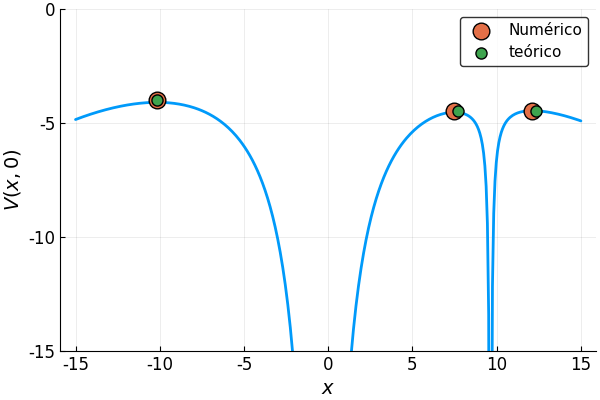
\includegraphics[width=0.8\linewidth]{pseudo_xaxis}
 \caption{Proyección del pseudo-potencial en el eje $x$ para ver sus puntos de inflexión. Aparecen $L_1, L_2$ y $L_3$ calculados con (\ref{eq:3body_L123}) (verde) y numéricamente (naranja).}
 \label{fig:3body_pseudo_xaxis}
\end{figure}

Para obtener $L_4$ y $L_5$ es importante destacar que la fuerza centrífuga es, por definición, radial hacia afuera. En este sentido, en la dirección radial se deben balancear la fuerza centrífuga con la gravitacional. Ésto hace que el balance en la dirección tangencial sea debido únicamente a los dos cuerpos primarios interactuando bajo sus campos gravitacionales. Para ésto, se proyecta la fuerza hacia sus direcciones radiales y tangenciales con los vectores $\mathbf{r}_{\parallel} = (x,y)$ y $\mathbf{r}_{\bot} = (-y,x)$. Así
\begin{align*}
 F_{\bot} &= \frac{1}{r_{\bot}} \mathbf{r}_{\bot} \cdot \mathbf{F} = \frac{y}{r_{\bot}} \left( - \frac{(1-\mu)(x + \mu)}{ r_{1,3}^3 } - \frac{\mu(x - 1 +\mu )}{ r_{2,3}^3 } + \frac{(1-\mu)x}{ r_{1,3}^3 } + \frac{\mu x}{ r_{2,3}^3 } \right) \\
 \therefore F_{\bot} &= \frac{ \mu(1-\mu) y}{r_{\bot}} \left( \frac{1}{r_{1,3}^3} - \frac{1}{r_{2,3}^3} \right),
\end{align*}
es decir, la condición para que la componente tangencial de la fuerza se anule es que ambos cuerpos estén a la misma distancia de la partícula $m_3$, lo cual tiene sentido ya que el sistema tiene el origen en el centro de masa entre $M_1$ y $M_2$. 

Para la componente radial, tenemos que
\begin{align*}
 F_{\parallel} &= \frac{1}{r_{\parallel}} \mathbf{r}_{\parallel} \cdot \mathbf{F} = \frac{1}{r_\parallel} \left( (x^2 + y^2) -  (1-\mu) \left( \frac{(x+ \mu)x}{r_{1,3}^3} + \frac{y^2}{r_{1,3}^3} \right) - \mu \left( \frac{(x - 1 +\mu) x}{r_{2,3}^3} + \frac{y^2}{r_{2,3}^3} \right) \right),
\end{align*}
pero $r_{1,3} = r_{2,3}$, por lo que lo anterior se simplifica a 
\begin{align*}
 F_{\parallel} = \frac{x^2 + y^2}{r_\parallel} \left( \frac{1}{R^3} - \frac{1}{r_{1,3}^3} \right).
\end{align*}

Encontramos así que $r_{1,3} = r_{2,3} = R$. $L_4$ y $L_5$ forman un tríangulo equilátero de lado $R$, cuya base es la distancia entre $M_1$ y $M_2$. Así,
\begin{align}
 L_4 &= \left( \frac{1 - 2\mu}{2}, \frac{\sqrt{3}}{2} \right), \\
 L_5 &= \left( \frac{1 - 2\mu}{2} , -\frac{\sqrt{3}}{2} \right),
 \label{eq:L4_L5}
\end{align} 
tal como se ve en la Figura \ref{fig:L_diagram}.

%FIGURA! 
\begin{figure}[h!]
 \centering
 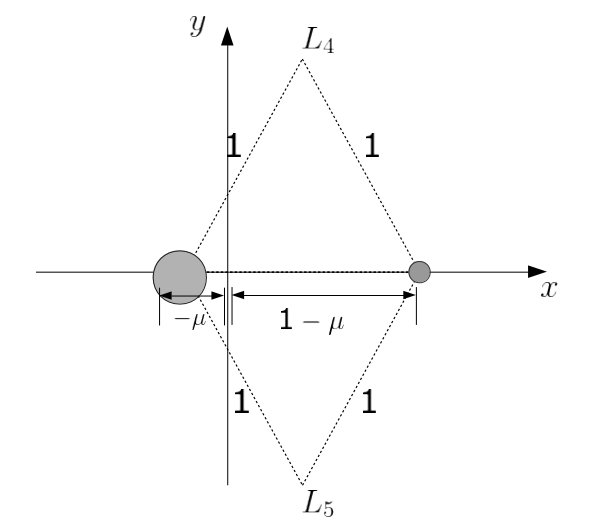
\includegraphics[width=0.8\linewidth]{lag_triangular}
 \caption{Diagrama que muestra la posición de $L_4$ y $L_5$ en unidades normalizadas donde $R=1$, $M_1 + M_2 = 1$.}
 \label{fig:L_diagram}
\end{figure}

La estabilidad de éstos puede estudiarse viendo cómo se comportan las ecuaciones de primera variación alrededor de los puntos de equilibrio, tal como se hace en \cite{Cornish1998}. Para esto basta construir la matriz de estabilidad 
\begin{equation*}
 A(\mathbf{x}) = \begin{bmatrix}
  \pder{\mathbf{f}_1}{x_1}(\mathbf{x}) & \dots & \pder{\mathbf{f}_1}{x_n}(\mathbf{x}) \\
  \vdots & \ddots & \vdots \\ 
  \pder{\mathbf{f}_n}{x_1}(\mathbf{x}) & \dots & \pder{\mathbf{f}_n}{x_n} (\mathbf{x})
\end{bmatrix},
\end{equation*}
donde $\dot{\mathbf{x}} = \mathbf{f}(\mathbf{x})$ y encontrar los eigenvalores de ésta para determinar qué tipo de punto singular se trata. Para este caso
\begin{equation}
 A(\mathbf{x}_{L_i}) = \begin{bmatrix}
  0 & 0 & 1 & 0 \\
  0 & 0 & 0 & 1 \\ 
  \pder{\dot{v_x}(\mathbf{x}_{L_i})}{x} & \pder{\dot{v_x}(\mathbf{x}_{L_i})}{y} & 0 & 2 \Omega \\
  \pder{\dot{v_y}(\mathbf{x}_{L_i})}{x} & \pder{\dot{v_y}(\mathbf{x}_{L_i})}{y} & -2\Omega & 0
\end{bmatrix},
\label{eq:stability_CR3BP}
\end{equation}
la cual será evaluada en los puntos lagrangianos $\mathbf{x}_{L_i}$, donde 
\begin{align}
 \pder{\dot{v}_x}{x} &=  1 - \frac{1-\mu}{r_{1,3}^3} + 3\frac{(1-\mu)(x + \mu)^2}{r_{1,3}^5} - \frac{\mu}{r_{2,3}^3} + 3\frac{\mu(x - 1 + \mu)^2}{r_{2,3}^5}, \nonumber \\ 
 \pder{\dot{v}_y}{y} &= 1 - \frac{1-\mu}{r_{1,3}^3} + 3\frac{(1-\mu)y^2}{r_{1,3}^5} - \frac{\mu}{r_{2,3}^3} + 3\frac{\mu y^2}{r_{2,3}^5}, \nonumber \\
 \pder{\dot{v}_x}{y} &= \pder{\dot{v}_y}{x} = 3 y \left( \frac{(1-\mu)(x+\mu)}{r_{1,3}^5} + \frac{\mu (x - 1 + \mu)}{r_{2,3}^5} \right),
 \label{eq:3body_stability}
\end{align}
con $r_{i,3}$ la distancia a $M_i$.

Para $L_1$, $L_2$ y $L_3$ se puede mostrar que son equilibrios inestables sin importar el valor de los cuerpos masivos \cite{MirelesJames2006}. De hecho, sustituyendo para $L_1$ y $L_2$ se obtiene
\begin{align*}
 \lambda_\pm &= \pm  \sqrt{1 + 2\sqrt{7}}, \\
 \sigma_\pm &= \pm i \sqrt{2\sqrt{7} - 1},
\end{align*}
mientras que en $L_3$ obtenemos 
\begin{align*}
 \lambda_\pm &= \pm \sqrt{ \frac{3(1 - \mu)}{8\mu} }, \\
 \sigma_\pm &= \pm i \sqrt{7},
\end{align*}
donde $\lambda_\pm \in \mathbb{R}$ en ambos casos, lo cual representa sillas en el espacio de configuraciones.

Sustituyendo $L_4$ y $L_5$ en (\ref{eq:3body_stability}), se obtiene que $\pder{\dot{v}_x}{x} = \pm \frac{3}{4}$, $\pder{\dot{v}_y}{y} = \pm \frac{9}{4}$ y $\pder{\dot{v}_x}{y} = \pm \frac{3\sqrt{3}}{2} (1-2\mu) $, cuyos eigenvalores son
\begin{align*}
 \lambda_\pm = \pm \frac{i}{2} \sqrt{ 2 - \sqrt{27(1-2\mu)^2 - 23} }, \\
 \sigma_\pm = \pm \frac{i}{2} \sqrt{ 2 + \sqrt{27(1-2\mu)^2 - 23} }.
 \end{align*}

Estos puntos serán estables si sus eigenvalores son puramente imaginarios, cuya condición se cumple si 
\begin{align*}
 2 &\geq \sqrt{27(1-2\mu)^2 - 23}, \\
 23 &< 27(1-2\mu)^2.
\end{align*}
Lo primero es equivalente a que 
\begin{equation}
 \mu \leq \mu_c := \frac{1}{2} \left(1 - \sqrt{\frac{23}{27}} \right) \approx 0.0385,
 \label{eq:mu_critica}
\end{equation}
y lo segundo se da siempre que lo primero se cumple\footnote{Esto es equivalente a que la masa principal sea aproximadamente $25$ veces más masiva que la otra ($1/26 = 0.0384 \approx \mu_c$).}.

Así, vemos explícitamente la condición para la estabilidad de los puntos $L_4$ y $L_5$. 

\subsection{Curvas de velocidad cero}
\label{sec:zvc}

Un último análisis que vale la pena hacer son las curvas de velocidad cero (CV0). Éstas son el punto máxmimo de retorno para una energía dada en el espacio de configuraciones. Este estudio se guía de las notas de Mireles en \cite{MirelesJames2006}. Podemos pensar, como analogía, que para una energía potencial dada, una partícula en caída libre no podrá rebotar más alto que cierta altura $h$ de la cual empezó. De hecho, justo cuando la partícula alcance dicha altura, su velocidad será idénticamente cero y volverá a caer. 

Para encontrar estas curvas en el PC3C, se impone cierta energía de Jacobi $C_J$ y se traza la curva tal que la velocidad sea cero, i.e.,
\begin{equation*}
 (x,y,0,0) = \left\lbrace V \ | \  V = \frac{1}{2}C_J \right\rbrace.
\end{equation*}

Como en el ejemplo de caída libre, todas las trayectorias estarán atrapadas ``debajo'' de esta curva y restringe las secciones en las que $m_3$ se puede mover. 

%FIGURA! 
\begin{figure}[h!]
 \centering
 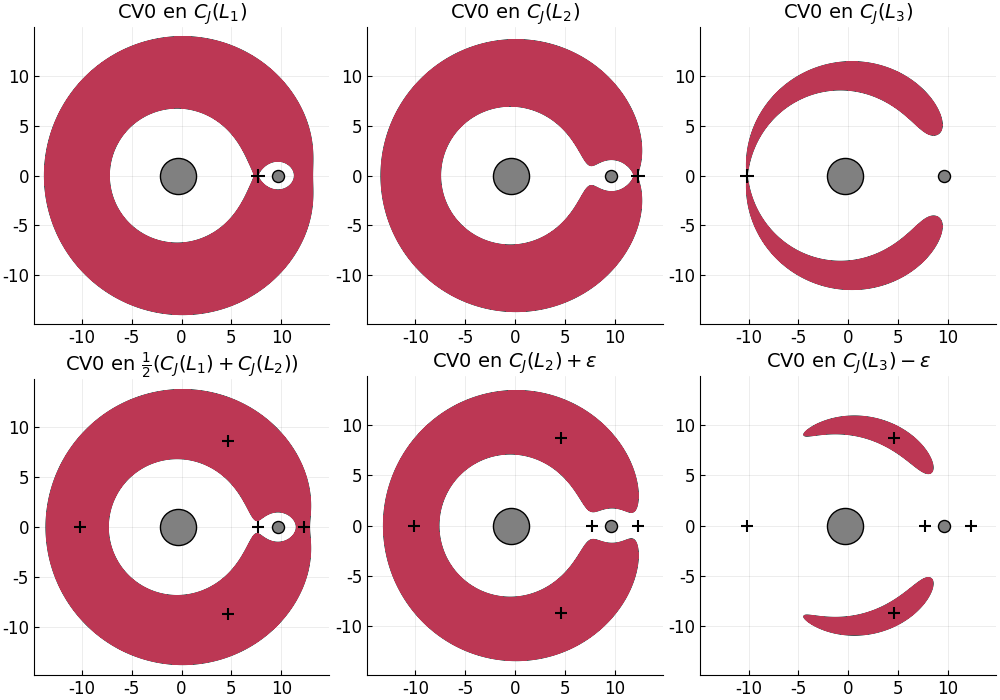
\includegraphics[width=0.9\linewidth]{zero_velocity_curves}
 \caption{\textit{Arriba:} CV0 sobre los puntos $L_1, L_2$ y $L_3$, respectivamente. \textit{Abajo:} CV0 sobre variaciones en energía sobre las de arriba, donde se tomó una variación respecto a la energía de Jacobi $\delta E = 0.05$. Se graficaron las energías mayores o iguales a la constante de Jacobi para ver la ``sección prohibida'' de las trayectorias. }
 \label{fig:zero_velocity_curves}
\end{figure}

La Figura \ref{fig:zero_velocity_curves} muestra algunas de estas curvas con consantes de Jacobi alrededor de $L_1$, $L_2$ y $L_3$ y algunas variaciones respecto a éstos. Al ser puntos tipo silla, dividen al espacio en regiones. El caso más interesantes está entre las energías de $L_1$ y $L_2$, ya que entre éstas se pueden diseñar condiciones iniciales que se queden siempre orbitando entre los dos planetas, o que se quede sólamente en uno de ellos.

La exploración del problema circular de tres cuerpos nos llevó a la adimensionalización de las ecuaciones de movimiento, resultando que éstas dependan únicamente del parámetro $\mu$, el estudio de los puntos lagrangianos y el tipo de equilibrio que tienen, y las CV0, que ayudan a determinar las secciones por las que $m_3$ se puede mover. Con ésto, las herramientas del TJ pueden encaminarse de una manera más eficiente, lo cual se hará a fondo en el próximo capítulo.